\section{LOFAR: The LOw-Frequency Array}

\pg
Our observations have all been made with the LOw Frequency Array LOFAR \citepads{2013A&A...556A...2V}. In this section, we describe its technical properties and its current state of the art. In particular, the distinction between ``Dutch" LOFAR and ``international" LOFAR - and the technical problems associated with each - will be made explicit in this section.

\pg
LOFAR is a SKA pathfinder instrument, which means that it serves not only as a cutting-edge instrument in its own right, but does so with the explicit aim of serving as testing grounds for technologies \& techniques which could be usefully implemented in the SKA. It is in this context, for example, that trailblazers such as NenuFAR \citepads{2012sf2a.conf..687Z}, a low-frequency extension of LOFAR, are tested. LOFAR is an interferometric array, with each of its elements made up of antennas combined into a phase array. It thus consists of antennas which are combined to form stations, which are themselves distributed throughout the Netherlands and Europe.
\begin{figure}[h!] 
  \begin{minipage}[c]{0.45\linewidth}
    \centering
    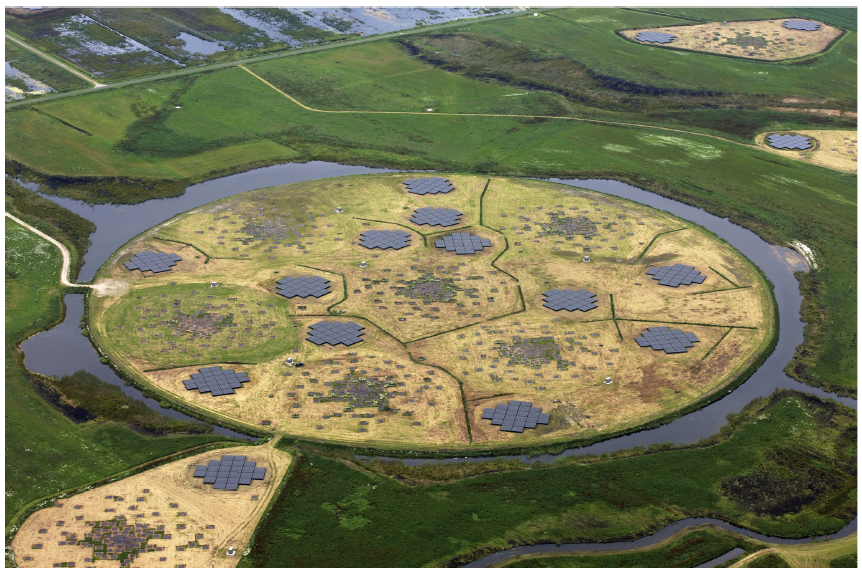
\includegraphics[width=\linewidth]{images/superterp.png}
	\subcaption{\label{fig.lofar.superterp} LOFAR core, known as the Superterp.}
%    \vspace{4ex}
  \end{minipage}
  \hfill
  \begin{minipage}[c]{0.45\linewidth}
    \centering
    \includegraphics[width=.5\linewidth]{images/{lofar-core-map_grey.jpg}}
    \subcaption{\label{fig.lofar.core} Distribution of the so-called LOFAR "core" stations, which include the Superterp.}
%    \vspace{4ex}
  \end{minipage} 
  \begin{minipage}[c]{0.45\linewidth}
    \centering
    \includegraphics[width=\linewidth]{images/{Distribution_Remote_Stations}} 
    \subcaption{\label{fig.lofar.remote} LOFAR with both "core" and "remote" stations.}
%    \vspace{4ex}
  \end{minipage}
  \begin{minipage}[c]{0.45\linewidth}
    \centering
    \includegraphics[width=.9\linewidth]{images/{Distribution_International_Stations}} 
    \subcaption{\label{fig.lofar.international} International LOFAR. Newer stations (one in Ireland, three in Poland) are not shown here.}
%    \vspace{4ex}
  \end{minipage} 
\caption{\label{fig.lofar.distribution} Geographic location and distribution of LOFAR stations, explicitly showing what is meant by Superterp, core, remote and international stations. All images from \href{https://www.astron.nl/radio-observatory/astronomers/users/technical-information/lofar-array-configuration/lofar-array-conf}{the official ASTRON website}}
\end{figure}


\pg
There are two bands to LOFAR, which are known as LOFAR-HBA (High-Band Antennas) and LOFAR LBA (Low-Band Antennas). \cref{fig.lofar.superterp,fig.fr606.layout} show the layout of the 6 innermost core stations and the French international LOFAR station, respectively.
\begin{figure}[h!]
\includegraphics[width=0.5\textwidth]{images/{LOFAR_NenuFAR.jpg}}
\caption{\label{fig.fr606.layout} Layout of FR606, the French LOFAR station at Nancay. At bottom left are the HBA tiles, bottom right the LBA dipoles, and at the top are some of the NenuFAR tiles.}
\end{figure}



\pg
We see the presence, in both cases, of two very different antenna types. One of these antenna types is not a single antenna, but rather a phased array: 16 antenna dipoles distributed in a $4 \times 4$ array. International LOFAR stations include 48 such tiles, distributed in a ``filled-disk" pattern, where the disk fill ratio is determined by the size of the tile. This pattern is shown in \cref{fig.hba.tile}. Dutch ``remote" stations have 96 such tiles spread in 2 disks (HBA\textunderscore INNER and HBA\textunderscore OUTER), while ``core" station HBA tiles are split into two 24-tile crosses. The antennas from each tile are combined into a phased array with a single ``tile beam", and all tile beams are themselves combined as a phased array into a station beam\footnote{Referece: \href{https://www.astron.nl/radio-observatory/astronomers/technical-information/antennae/antennae-description}{ASTRON technical description}}. This station beam is then pointed digitally.
\begin{figure}[h!]
\includegraphics[width=0.45\textwidth]{images/{Schematic-diagram-of-a-24-tile-LOFAR-HBA-station-A-tile-is-made-of-16-dual-polarization.png}}
\caption{\label{fig.hba.tile} Layout of a single HBA tile. Source: \href{https://www.researchgate.net/profile/Sarod_Yatawatta/publication/281316394/figure/fig1/AS:614002589720576@1523401033149/Schematic-diagram-of-a-24-tile-LOFAR-HBA-station-A-tile-is-made-of-16-dual-polarization.png}{Sarod Yatawatta researchgate profile}}
\end{figure}

\pg
LOFAR-HBA is sensitive to higher frequencies, from 120 MHz to 240 MHz\footnote{Reference: \href{http://www.lofar.org/about-lofar/system/lofar-numbers/lofar-numbers}{LOFAR.org website}}. It has a smaller field of view than LOFAR-LBA, but a better angular resolution. 

\pg
LBA antennas, meanwhile, follow a very simple - and cost-effective - design. A typical LBA antenna is shown in \cref{fig.lba.ant}. 96 such antennas are spread in a semi-random pattern in each LOFAR station\footnote{Reference: \href{http://www.lofar.org/about-lofar/system/lofar-numbers/lofar-numbers}{LOFAR.org website.}}. In Dutch stations, 48 of these are used at all times. They are combined as a single phased array.
\begin{figure}[h!]
\includegraphics[width=0.45\textwidth]{images/{lba.png}}
\caption{\label{fig.lba.ant} Picture of a single LBA antenna. Source: \href{https://i2.wp.com/lofar.ie/wp-content/uploads/2017/04/lba.png?resize=1500\%2C1000}{LOFAR technology website.}}
\end{figure}

\pg
The dipole design frees observers from the need to physically point antennas at all: the final station pointing is achieved by digitally introducing delays in observed phase before averaging the data. In this sense, the pointing is achieved in a similar way as individual HBA tile pointing, albeit in analog. These antennas are receptive to signals emitted in the 30-80 MHz frequency range.

\pg
At the time of writing, use of the LBA data is still relatively new, as its calibration is a very tricky problem. For similar reasons, international LOFAR (i.e. the full LOFAR array) has not been used, at the time of writing, to create wide-field survey images. A large part of the work described in this manuscript consists of reaching a point where full use can be made of international LOFAR, in a streamlined and repeatable way. 

